\documentclass[12pt]{article}
\usepackage[portuguese]{babel}               % acentos e tal
\usepackage[utf8]{inputenc}                  %
\usepackage{amsmath}						 % math

\usepackage{amsfonts}						 % math symbols (ex: R^n)
\usepackage{amssymb}

\usepackage{graphicx}						 % imagens
\usepackage{hyperref}                        % hyperlink
\usepackage[usenames, dvipsnames]{color}
% \usepackage[]{algorithm2e}
\usepackage{algpseudocode}
\usepackage[numbered, framed]{mcode}
\usepackage{listings}
\lstdefinestyle{term}
{
    backgroundcolor=\color{black},
    basicstyle=\footnotesize\color{white}\ttfamily
}

\algrenewcommand\Return{\State \algorithmicreturn{} } % tirar os returns da mesma linha nos pseudocodigos 
\usepackage{indentfirst}
\usepackage{enumitem}
\setlist[description]{leftmargin=\parindent,labelindent=\parindent}

% cores
\definecolor{title_color}{RGB}{60, 100, 200}
\definecolor{text_color}{RGB}{0, 0, 0}
\definecolor{section_color}{RGB}{25, 100, 75}
\definecolor{basic_dir}{RGB}{0, 255, 170}
\definecolor{svb}{RGB}{0, 50, 150}

% títulos
\usepackage{titlesec}
\titleformat*{\section}{\LARGE\bfseries}

\usepackage{helvet}
\renewcommand{\familydefault}{\sfdefault}

\title{Relatório EP3 MAC315}

\author{Bruno Sesso, Gustavo Estrela de Matos}

\bigskip
\date{\today}

\begin{document}
\begin{titlepage}

\begin{center}
	\begin{flushleft}
    	\textcolor{title_color} {
        	\fontsize{1cm}{1em}\selectfont {Implementação do Método Simplex\\}
    	}
    \end{flushleft}
  
    \begin{flushleft}{
    \textcolor{text_color} {
    	\href{mailto:bsesso@gmail.com}{Bruno Sesso} 8536002\\    					      		           \href{mailto:estrela.gustavo.matos@gmail.com}{Gustavo Estrela de Matos} 8536051\\}
    }
    \end{flushleft}
   
	\today
\end{center}
\end{titlepage}

\newpage
\section{Introdução}



\subsection{Apresentação do problema}
    Os problemas de Programação Linear (PL) são casos específicos de otimização combinatória em que a função objetivo e as restrições são ambos lineares. Portanto a função objetivo é da forma $c^{T}x$ e as restrições são da forma $a_{i}^{T}x \geq b_{i}$ ou $a_{i}^{T}x \leq b_{i}$, com $c, x, a_i \in \mathbb{R}^{n}$ e $b_{i} \in \mathbb{R}$.
    
    Multiplicando por $-1$ todas as restrições da forma $a_{i}^{T}x \geq b_i$, podemos escrever qualquer PL como:

    \begin{center}
    	\begin{tabular}{r l}
        	minimizar & $c^Tx$ \\
        
	        sujeito a & $Ax \leq b$, \\
        
        			  & $A \in R^{m \times n}$ e $b \in \mathbb{R}^m$.
		\end{tabular}
    \end{center}
	Também é possível mostrar que qualquer PL pode ser escrito na forma: 

	\begin{center}
    	\begin{tabular}{r l}
	  		minimizar & $c^Tx$ \\
        
	        sujeito a & $Ax = b$, \\
       				  & $x \geq 0$~\cite{315book}.
        \end{tabular}
    \end{center}
    Se for escrito dessa maneira, dizemos que o problema está no formato padrão. Adotaremos esse formato durante todo o trabalho.
    
    Se vale que $Ax^1 = b$ e $x^1 \geq 0$ dizemos que $x^1$ é um ponto viável. O conjunto $P = \{x| Ax = b, x \geq 0\}$ de todos os pontos viáveis é chamado conjunto viável.
    
    Uma solução ótima do problema é um ponto $x^1 \in P$ que minimiza \footnote[1]{Se o interesse for maximizar ${c}^{T}x$, podemos simplismente conseguir um problema equivalente em que o objetivo seja minimizar $-{c}^{T}x$.} a função objetivo $c$. Se $x^1$ existe, dizemos que o custo ótimo é $c^Tx$. Se $x^1$ não existe, ou não existem pontos viáveis ($P = \emptyset$), ou podemos diminuir o custo o quanto quisermos e dizemos que o custo ótimo é $- \infty$.
    

\subsection{Objetivos do trabalho}
	Neste trabalho, temos o objetivo de desenvolver, na linguagem Octave, o algoritmo simplex para resolver problemas de Programação Linear.


\section{Conceitos fundamentais}
	Antes de introduzirmos o funcionamento do nosso algoritmo, precisamos definir alguns conceitos que são fundamentais para garantir sua corretude.

	Seja o nosso problema de Programação Linear o seguinte:
    \begin{center}
    	\begin{tabular}{r l}
	  		minimizar & $c^Tx$ \\
        
        	sujeito a & $Ax = b$ \\
            & $x \geq 0$ \\
       	
        
        com & $c, x \in \mathbb{R}^n$, $A \in \mathbb{R}^{m \times n}$ e $b \in \mathbb{R}^{m}$.
        \end{tabular}
    \end{center}

	Além disso, vamos usar a notação $a_i$ para a i-ésima linha de A e $A_i$ para a i-ésima coluna de A.
    
    
\subsection{Restrições e degenerecência}
	Uma restrição $a^{T}_{i}x \geq b_{i}$ (ou $a^{T}_{i}x \leq b_{i}$), com $a_{i} \in \mathbb{R}^{n}$ e $b_i \in \mathbb{R}$, é uma \emph{restrição ativa} em um ponto $x^1 \in \mathbb{R}^n$ se $a^{T}_{i}x^1 = b_i$. Uma restrição de igualdade é sempre ativa. Um conjunto de restrições será dito LI se os vetores $a_{i}$ correspondentes forem LI.
    
    Diremos que $x^1$ uma solução viavel básica é \emph{degenerada} se existem mais de $n$ restrições ativas LI nesse ponto. Como as $m$ restrições de igualdade são sempre cumpridas, temos que as soluções básicas degeneradas possuem mais do que $n - m$ componentes nulas, enquanto que as não degeneradas possuem exatamente $n - m$.
    
    
\subsection{Soluções Viáveis Básicas}
	\label{subsec:svb}
    Dizemos que um ponto $x \in \mathbb{R}^{n}$ do conjunto viável $P$ é uma \emph{solução viável básica}, se existem $n$ restrições ativas em $x$ que são LI. Note que para problemas no formato padrão, existem sempre $m$ restrições ativas LI vindas de $Ax = b$, e as outras $n - m$ vem, necessariamente de $x \geq 0$. Portanto, uma solução viável básica possui ao menos $n - m$ componentes nulas.
    
    Se $x^1$ é uma solução básica não degenerada e seja $B(1), ..., B(m)$ os índices das componentes não nulas de $x$. A matriz $B = \begin{bmatrix} A_{B(1)}, ..., A_{B(m)}\end{bmatrix}$ é chamada \emph{matriz básica} associada a $x^1$.
    
    %teorema 2.8
    Se o conjunto $P$ tem uma solução viável básica, então ou o custo ótimo é $- \inf$ ou existe $x^1 \in P$ solução viável básica que é ótimo, ou seja, o custo de qualquer ponto do conjunto viável é maior ou igual do que o custo de $x^1$. Portanto, na solução de um PL com ao menos uma solução viável básica, podemos limitar a esses elementos a nossa busca por um ponto de custo ótimo~\cite{315book}.
    
    
\subsection{Direções básicas}
	Se $x^1$ é um solução viável básica de $P$, com índices básicos $B(1), ..., B(m)$. Dizemos que $d \in \mathbb{R}^n$, tal que $d_j = 1$, $Ad = 0$ $(A(x + \theta d) = b)$ e $d_i = 0$ para todo $i \notin \{B(1), ..., B(m)\}$, é a j-ésima direção básica partindo de $x^1$. Seja $d_B = \begin{bmatrix}d_{B(1)}, ..., d_{B(m)}\end{bmatrix}$, como $A(x + \theta d) = b$, temos que $d_B = -B^{-1}A_j$. Usaremos $u = -d_B = B^{-1}A_j$ por facilidade de notação, durante o trabalho.
 
 
	A figura \ref{fig:basic_dir} dá um exemplo de direções básicas, $di$ e $dj$ a partir de uma solução viável básica $x^1$. Note que o poliedro pode ou não limitar um $\theta$ tal que o ponto $y = x^1 + \theta*d$ ($d$ direção básica) seja viável, e como veremos em \ref{concepts:adj_svb} isso pode implicar em custo $-\infty$ se nessa direção o custo diminui.
    
\thicklines    
\begin{center}\label{fig:basic_dir}
    \begin{picture}(200, 200)
        \put(50, 50){\line(1, 0){100}}
        \put(50, 50){\line(-1, 1){50}}
        \put(35, 35){$x^2$}
        \put(50, 50){\circle*{5}}
        
        \put(-15, 85){\textcolor{svb}{$x^1$}}
        \put(0, 100){\line(1, 2){35}}
        % di
	    \put(0, 100){\textcolor{basic_dir}{\vector(1, 2){20}}}
		\put(5, 130){\textcolor{basic_dir}{$d_i$}}
        %dj
		\put(0, 100){\textcolor{basic_dir}{\vector(1, -1){25}}}
		\put(15, 65){\textcolor{basic_dir}{$d_j$}}
        \put(0, 100){\circle*{5}}
        
        \put(150, 50){\circle*{5}}
        \put(135, 35){$x^3$}
        
        \put(75, 100){$P$}
    \end{picture}
\end{center} 

\subsection{Custos reduzidos}\label{concepts:reduced costs}

    Seja $x^1$ uma solução viável básica, $B$ a matriz básica associada e $c_B = \begin{bmatrix} c_{B(1)}, ..., c_{B(m)}\end{bmatrix}$. Definimos, para cada $j \in \{1, ..., n\}$ o custo reduzido: 
    \begin{center}
    $\overline{c}_{j} = c_j - c_{B}^{T} B^{-1}A_j$.
    \end{center}
    
    %teorema 3.1
    Seja $x^1$ uma solução viável básica e $\overline{c}$ o vetor de custos reduzidos correspondente. Sabemos que se $\overline{c} \geq 0$, então $x^1$ é ótimo. Além disso, se $x^1$ for ótimo e não degenerado, então $\overline{c} \geq 0$~\cite{315book}. Portanto, se estivermos em uma solução viável básica e $\overline{c} \geq 0$, então estamos em um ponto ótimo.
    
    Note que ao escolhermos uma direção viável básica, o custo de um ponto $y = x^1 + \theta d_j$ é $c^{T}(x^1 + \theta d_j) = c^{T}x^1 + \theta (c_j - c^{T}_{B}B^{-1}A_j) = c^{T}x^1 + \theta \overline{c}$. Portanto, podemos dizer que o custo reduzido representa a variação do custo ao percorrer uma direção básica.

\subsection{Soluções Viáveis Básicas adjacentes}\label{concepts:adj_svb}
	Seja $x^1$ uma solução viável básica com índices básicos $B(1), ..., B(m)$. Uma solução viável básica é \emph{adjacente} a $x^1$ se compartilha $m-1$ índices com $x^1$. Para achar uma solução viável básica adjacente, vamos usar as direções básicas, pois elas forçam o crescimento de uma variável $j$ não-básica, mantendo $Ax = b$ e $x \geq 0$. Veremos que para um $\theta \geq 0$, o ponto $x^1 + \theta d_j$ é solução viável básica adjacente a $x^1$, com $d_j$ como foi definido em \ref{concepts:reduced costs}. 
    
    Vamos tomar $\theta = \min_{i = 1,...,m | u_i > 0}{\{x_{B(i)} / u_i\}}$ e ver que $x^2 = x^1 + \theta d_j$ é de fato uma solução viável básica adjacente a $x^1$. Caso todas as componentes de $u_i$ sejam menores ou igual a zero e o custo reduzido na direção $j$ menor do que zero teremos que o problema tem custo ótimo $- \infty$, como será explicado a seguir.
    
    Se $\theta$ definido acima não existe, temos que todas as componentes de $u_i$ são menores ou igual a zero ($d \geq 0$), logo qualquer ponto $x^2 = x^1 + \theta d$ é viável com $\theta \geq 0$, pois a restrição $Ax^2 = b$ é verificada (por construção), e $x^2_j = x^1_j + \theta \geq x^1_j \geq 0$, e para $i$ básico $x^2_j = x^1_j + \theta d_ j \geq x^1_j \geq 0$. Se ainda tivermos que o custo diminui nessa direção, poderemos diminuir o custo o quanto quisermos e a solução do problema será $- \infty$.
    
    Se $\theta \in \mathbb{R}$, como $d_i = 0$ $\forall{i \in \{B(1), ..., B(m)\}, i \neq j}$, temos que para essas mesmas componentes $x^2$ é nulo. Logo, temos $n - 1$ restrições ativas LI em $x^2$. Suponha que para $l \in \{1,..,m\}$ vale que $\theta =  x_{B(l)} / u_l$, então $x^2_{B(l)} = x^1_{B(l)} + (-x^1_B(l)/d_{B(l)}) * d_{B(l)} = 0$ (diremos que $B(l)$ sai da base), logo existem $n$ restrições ativas LI em $x^2$. Além disso, por construção, vale que $Ax = b$ e $x \geq 0$ para variáveis não básicas e para $x_B(l)$. Para $B(k)$ básico diferente de $B(l)$, temos que $x^2_B(k) \geq x^1_{B(k)} + (-x^1_B(k)/d_{B(k)}) * d_{B(k)} = 0$. Portanto $x^2$ é solução viável básica adjacente a $x^1$ e, como a base de $x^2$ é $\{B(1), ..., B(l - 1), j, B(l + 1), ..., B(m)\}$, $x^2$ é adjacente a $x^1$.
    
    
    
\section{Fase 1 do simplex}
	Para iniciar a fase 2 do algoritmo simplex precisamos de uma solução viável básica $x^1$, a sua base associada e a inversa da matriz básica. Nesta seção explicaremos o funcionamento da fase 1 do método simplex, responsável por descobrir estes parâmetros.

Para descobrir esses parâmetros vamos criar um problema auxiliar de programação linear:

\begin{center}
	\begin{tabular}{r l}
		minimizar & $\sum_{i = 1}^{m} y_i$ \\
		sujeito a & $
					[\begin{array}{c | c}
						A & I
					\end{array}]
					
					\bigg[\begin{array}{c}
						x \\
						\hline
						y
					\end{array}\bigg]
					
					\leq b$, \\
			com   &	$A \in R^{m \times n}$; $b, y \in \mathbb{R}^m$; $I \in \mathbb{R}^{m \times m}$ \\
            & $x, y \geq 0$
	\end{tabular}
\end{center}
Chamaremos as variáveis de $y$ aritificiais, e a matriz $[\begin{array}{c | c} A & I	\end{array}]$ de $\overline{A}$.

Note que o ponto $[\overbrace{0, ..., 0}^{n}|b]$ é uma solução viável básica do problema auxiliar, assumindo $b \geq 0$, com índices básicos $n + 1, ..., n + m$ e matrix básica $B = I$. Portanto, temos os parametros necessários para embalar a fase 2 do simplex para o problema auxiliar.

Assumimos no último parágrafo que $b \geq 0$. É fácil verificar que isso não implica em uma perda de generalidade, pois, se $b_i < 0$, basta multiplicar a $i$-ésima restrição por $-1$.



\subsection{Custo ótimo do problema auxiliar e viabilidade do problema original}
\label{fase2:custo_otimo}
Observe que qualquer ponto viável do problema tem custo maior ou igual a zero. Além disso, se existe uma solução viável $x^1$ do problema original, o ponto $[x^1 | 0, ..., 0]$ é uma solução viável com custo zero, portanto com custo ótimo. Sendo assim, temos que se o problema original possui solução viável, então o problema auxiliar tem custo ótimo igual a zero. Na contra-positiva, se acharmos uma solução ótima para o problema auxiliar com custo diferente de zero, então o problema original é inviável.


\subsection{Solução do problema auxiliar}
Como o custo do problema auxiliar é sempre maior ou igual a zero, o custo ótimo nunca será $-\infty$, portanto a fase 2 sempre descobrirá alguma solução viável básica ótima. Se o custo dessa solução for maior que zero, o problema original é inviável, como explicado na seção \ref{fase2:custo_otimo}. Se o custo for zero, a solução do problema auxiliar $[x|y] = [x | 0, ..., 0]$ também será uma solução do problema original. 

Porém, mesmo que $[x | 0, ..., 0]$ seja uma solução viável básica do problema original, é possível que a base dada pela fase 2 do problema auxiliar tenha índices das variáveis artificiais, que serão eliminadas para iniciar a fase 2 para o problema original. Veremos na \hyperref[rm_artificiais]{proxima seção} como remover os índices ariticiais da base.

\subsection{Remoção de índices artificiais da base}
\label{fase2:rm_artificiais}
Suponha que temos um índice $l > m$ aritificial que esteja na base. Queremos tirá-lo da base e adicionar um índice $j \leq m$ na base. Veremos agora, como descobrir tal índice e como mudar a base.

Suponha, sem perca de generalidade, que apenas os $k < m$ primeiros indices básicos não são de variáveis artificiais. Para o índice $j$ na base, devemos garantir que $A_{j}$ é LI com $\{A_{B(1)}, ..., A_{B(k)}\}$. Suponha que a matriz básica é $B$ e que queremos remover a $l$-ésima variável da base, por ser atificial. Veja que $B^{-1}A_{B(i)} = e_i$ para $1 \leq i \leq k$, portanto, basta escolher $j$ não artificial tal que $(B^{-1}A_j)_l = A_j  \neq 0$ e teremos garantia de que estamos escolhendo uma coluna LI para formar a base.

Se não ouver $j$ como descrito acima, teremos que $(B^{-1}A_j)l = 0$ para todo $1 \leq j \leq m$. Veja que se $g^T$ é a $l$-ésima linha de $B^{-1}$, então $g^TA = 0$, ou seja, $g_1a_1 + ... + g_ma_m = 0$, portanto as linhas de $A$ são LD e podemos então, eliminar a $l$-ésima linha de $A$ do nosso problema \cite{315book}.

Veja abaixo o pseudocódigo para remoção de índices artificiais da base:
\bigskip

\begin{algorithmic}
\Function{$RemoveAritificiais$}{$A$, $I$, $B^{-1}$, $m$, $n$}
	\ForAll{$\{ l \in \{B(1), ..., B(m)\} | l > n\}$}
		\State $candidates \gets \{i \in I.n | i< n\}$
		\State $x \gets length(candidates)$
		\State $k \gets 1$;
		\While{$k \leq x$ and $B^{-1}_lA_{I.n(candidates(k))}$} 
			\State $k \gets k + 1$
		\EndWhile
		\If{$k > x$}
			\State $m \gets m - 1$
			\State remova $l$-ésima linha e $l$-ésima coluna de $B$
			\State remova $l$-ésima linha de $A$
			\State remova a $l$-ésima entrada de $I.b$
			\State remova a $l$-ésima entrada de $b$
		\Else
			\State $u \gets B^{-1}A_k$ 
			\State $atualizaBase(I, invB, u, l, k, m)$
		\EndIf 
	\EndFor
\EndFunction
\end{algorithmic}
	
\section{Pseudocódigo do algoritmo simplex}
\begin{algorithmic}
\Function{$Simplex$}{$A$, $b$, $c$, $m$, $n$}
	\ForAll{$i | b_i < 0$}
		\State $b_i \gets b_i * -1$
	\EndFor
	\State $A \gets [A | I]$, $I \in \mathbb{R}^{m \times m}$
	\State $x \gets [\vec{0}, b]$, $\vec{0} \in \mathbb{R}^{n}$
	\State $c1 \gets [\vec{0}, \vec{ac}]$, $\vec{ac} = [1, ..., 1] \in \mathbb{R}^m$
	\State $I.b \gets [n + 1, ..., n + m]$
	\State $I.n \gets [1, ..., n]$
	\State $B^{-1} = I$, $I \in \mathbb{R}^{m \times m}$
	\State $(ind, x, d, I, B^-1) = fase2(A, b, c1, m, n + m, x, I, B^{-1})$
	\If{${c1}^{T}x > 0$}
		\Return $(1, NIL, NIL)$
		\Comment{Problema inviável}
	
	\EndIf
	\State $(I, A, invB, m) \gets removeArtificials (A, I, invB, m, n, b)$
	\State $x \gets [x_1, ..., x_n]$
	\State $(ind, x, d, I, B^-1) = fase2(A, b, c, m, n, x, I, B^{-1})$
	\If{$ind = -1$}
		\Return $(-1, x, d)$
		\Comment{Custo ótimo = $-\infty$}
	\Else
		\Return $(0, x, d)$
		\Comment{Solução ótima encontrada}
	\EndIf
\EndFunction
\end{algorithmic}

\section{O algoritmo}

\subsection{Objetivo}
	Nossa motivação é solucionar um problema de programação linear (\emph{PL}) que consiste em minimizar uma função linear (função de custos) sujeita a restrições lineares. Agora que temos os conceitos necessários, vamos desenvolver um algoritmo para solucionar tal problema.

\subsection{O que temos a princípio}
\label{fase2:args}
	Dado o problema:
    \begin{center}
    	\begin{tabular}{r l}
	  		minimizar & $c^Tx$ \\
        
        	sujeito a & $Ax = b$ \\
            & $x \geq 0$ \\
        \end{tabular}
    \end{center}
  
	Queremos achar o $x$ que satisfaça todas as restrições e minimize $c^Tx$. Portanto temos como informação inicial: 
	\begin{description}
		\item[$A$:] Matriz $m \times n$ de restrições
		\item[$b$:] Vetor de dimensão $m$
        \item[$c$:] Vetor de custos de dimensão $n$
        \item[$m$:] Número de restrições de igualdade
        \item[$n$:] Número de variáveis
	\end{description}

    Logo nossa função que calcula $x$ terá a seguinte forma: \\
    \begin{center}
    \texttt{simplex(A, b, c, m, n)}
    \end{center}

\subsection{O que recebemos no final}
    Como já vimos antes, temos três possíveis cenários de resultados da nossa função:
    \begin{enumerate}
        \item O problema é inviável, portanto não existe solução ótima
        \item Existe solução ótima, logo o custo ótimo é um valor finito
        \item O custo ótimo é $-\infty$, e não existe solução ótima
    \end{enumerate}
    Logo, nossa função deve retornar informação suficiente para sabermos em qual dos três casos estamos e os valores relevantes para cada um. Com isso em mente, nossa função tem o seguinte esqueleto:
    \begin{center}
        \texttt{[ind x d] = simplex(A, b, c, m, n)}
    \end{center}
    Onde:
    \begin{center}
    \begin{tabular}{ c  c  c  c }
        \textbf{Caso} & $ind$ & $x$  & $d$ \\  \hline
        1    & 1   & vetor vazio & vetor vazio \\
        2    & 0   & solução ótima & vetor vazio \\
        3    & -1  & ultima svb computada & direção que vai a $-\infty$ \\
    \end{tabular}
    \end{center}

\subsection{A função simplex}
    Nos preocupando somente com o caso onde o problema tem solução, nosso algortimo seria algo próximo do seguinte: 

    \begin{algorithmic}
    \Function{$simplex$}{$A$, $b$, $c$, $m$, $n$}
        \State \texttt{multiplica restrições com $b < 0$ por -1}
        \State $A' \gets [\begin{array}{c | c} A & I \end{array}]$
        \State $x' \gets \bigg [\begin{array}{c} 0 \\ \hline b \end{array} \bigg]$
        \State $c' \gets \bigg [\begin{array}{c} 0 \\ \hline 1 \end{array} \bigg]$
        \State $B \gets \bigg [\begin{array}{c c c c} A_{B(1)} & A_{B(2)} & \dots & A_{B(m)} \end{array} \bigg ]$ \\
        \State $x$ $\gets$ \texttt{fase2}$(A', b, c', m, m + n, x')$ \\
        \State $x$ $\gets$ \texttt{fase2}$(A, b, c, m, n, x)$ 
        \Return{$x$}
    \EndFunction
    \end{algorithmic}

    Nota-se que o algoritmo é dividido em 3 partes:
    \begin{enumerate}
        \item Modificar problema inicial, adicionando $m$ variáveis artificiais
        \item Encontrar solução inicial para o problema inicial resolvendo o modificado
        \item Resolver o problema inicial
    \end{enumerate}
    Podemos resolver os dois problemas, dado uma solução inicial, graças a função \texttt{fase2} que resolve problemas de programação linear a partir de uma solução viável básica inicial. Imaginando que já temos essa função, nosso algoritmo final em octave é:

    \begin{lstlisting}
function [ind, x, d] = simplex(A, b, c, m, n)
    % Arruma restricoes para que b > 0
    for i = 1 : m
        if (b < 0)
            b *= -1;
            A(i, :)  *= -1;
        end
    end

    % Cria problema auxiliar para achar primeira solucao 
    % para o problema inicial
    A = [A, eye(m)];
    x = [zeros(n, 1); b];
    c1 = [zeros(n, 1); ones(m, 1)];
    I = struct('b', [n + 1 : n + m], 'n', [1 : n]);
    invB = eye(m);

    % Resolve problema auxiliar
    [ind, x, d, I, invB] = fase2(A, b, c1, m, n + m, x, I, invB);

    if x(n + 1 : n + m) != 0
        % Problema Inviavel
        ind = 1;
        x = [];
        d = [];
        return;
    end

    % Remove vaiaveis artificiais da base. (nao altera x)
    [I, A, invB, m] = removeArtificials(A, I, invB, m, n, b);
    x = x(1 : n);


    % Resolve problema inicial, com solucao encontrada
    [ind, x, d, I, invB] = fase2(A, b, c, m, n, x, I, invB);
    \end{lstlisting}

	
	Utilizamos uma estrutura chamada de $I$ que guarda os índices básicos e não básicos, representados respectivamente pelos vetores $I.b$ e $I.n$. Nessa implementação, é fácil ver a correspondência entre as principais etapas vistas quando apresentamos o pseudocódigo. Entre as linhas \texttt{3} e \texttt{16} modificamos o problema original, nas linhas de \texttt{19} a \texttt{31} encontramos uma solução inicial e na linha \texttt{35} resolvemos o problema.
    
    Uma das melhorias feita para reduzir o espaço utilizado foi armazenar $A'$ e $x'$ (do pseudocódigo) em $A$ e $x$ respectivamente. Ainda assim, há certo desperdício de espaço utilizado em funções, pois o octave não envia argumentos por referência. Ou seja, quando enviamos $invB$ para \texttt{fase2}, por exemplo, ao modifica-la dentro da função, o octave cria uma cópia e então altera seus valores. Poderiamos ter feito alterações para que não haja esse tipo de desperdício, mas optamos por um código mais legível e modularizado.
    
    Visando melhorar nosso desempenho, passamos e retornamos alguns argumentos extras nas funções \texttt{fase2} e \texttt{removeArtificials}. Dessa forma, evitamos cálculos desnecessários de $B^{-1}$ e dos indices básicos associados à solução $x$. Nos poupar o cálculo de $B^{-1}$ é uma melhoria significativa, visto que isso tem complexidade $O(n^3)$.


\subsection{fase2}
	A função \texttt{fase2} vista na seção anterior, é de grande importância para nosso algoritmo. Dada uma solução viável básica inicial, essa função "anda" pelas soluções adjacentes, buscando uma na qual o custo calculado seja menor que na atual. Tendo a nova solução, voltamos a situação inicial e o algoritmo é executado novamente. Fazemos isso, tomando o cuidado para não andarmos em ciclos, até encontrar uma solução viável básica na qual todas as soluções adjacentes tem custo maior. Assim concluimos que essa solução é ótima. Tendo os conceitos da seção 2, produzimos o seguinte pseudocódigo:

\begin{algorithmic}
	\Function{$fase2$}{$A$, $b$, $c$, $m$, $n$, $x$}
		\State $\overline{c}^T \gets c^T - (c_B^T B^{-1})A_j$
		\While{$!(\overline{c} \geq 0)$}
			\State $j \gets j \not\in {B(1), \dots, B(m)}$, $t.q.$ $\overline{c}_j < 0$ \Comment Usando regra anti-ciclagem
			\State $u \gets B^{-1} A_j$
			\If{$u < 0$}
				\Return $(-1, d)$ \Comment Custo ótimo é $-\infty$
			\EndIf
			\State $\theta \gets \min_{u_l \geq 0} {\frac{x_{B(l)}}{u_l}}, l = 1, \dots, m$
			\State $x \gets x + \theta d$
			\State $B(l) \gets j$
			\State \Call{$atualiza$}{$invB$}
			\State $\overline{c}^T \gets c^T - (c_B^T B^{-1})A_j$
		\EndWhile
		\Return $(0, x)$
	\EndFunction	
\end{algorithmic}

	De forma muito similar, temos nosso algoritmo implementado em octave:
	\begin{lstlisting}
function [ind, x, d, I, invB] = fase2(A, b, c, m, n, x, I, invB)
    [redc, u, ij] = custoDirecao(A, invB, c, n, m, I);
    while redc < 0  % se essa condicao falha, x e otimo
        [imin, teta] = calculaTeta(x, u, I);
        if imin == -1  % custo otimo e -inf e u tem a direcao
            ind = -1;
            d = u2d(u, I.n(ij), I);
            return;
        end

        % atualiza
        x = atualizax(x, teta, u, I.n(ij), I); 
        [I, invB] = atualizaBase(I, invB, u, imin, ij, m);

        [redc, u, ij] = custoDirecao(A, invB, c, n, m, I);
    end
    
    d = [];
    ind = 0;
end 

    \end{lstlisting}

\subsection{Complexidade}
	A complexidade da função \texttt{simplex} depende basicamente da complexidade de \texttt{removeArtificials} e \texttt{fase2}. Primeiramente analisaremos a complexidade das funções auxiliares para então analisar as principais.

\subsubsection{Função custoDirecao}
A função custoDirecao é responsável por escolher uma direção básica $j$ com custo reduzido menor do que zero.
\begin{algorithmic}
\Function{$custoDirecao$}{$A, B^{-1}, c, n, m, I$}
	\State $j \gets 1$
	\While{$j \leq n - m$}
		\State $redc = c(I.n(j)) - c^T_BA_{I.n(j)}$
		\If{$redc < 0$}
			\State $ij \gets j$
			\State $u \gets B^{-1}A_{I.n(ij)}$
			\Return $(redc, u, ij)$
		\EndIf
		\State $j \gets j + 1$		
	\EndWhile
	\Return $(0, -1, NIL)$
\EndFunction
\end{algorithmic}

	Apesar de estar dentro do loop principal, $u \gets B^{-1}A_{I.n(ij)}$ é executada somente uma vez, pois assim que executada, logo em seguida uma chamada de retorno também é. Portanto essa linha leva $O(m^2)$, pois é multiplicação de uma matrix $m \times m$ por um vetor de dimensão $m$. Já a primeira linha de dentro do loop, leva $O(m)$, pois é produto de dois vetores de tamanho $m$. No entanto, essa linha é executada, no pior caso, $(n - m)$ vezes, isto é $O((n-m)m) = O(nm)$. Como $n > m$, a função como um todo tem complexidade $O(nm)$.

\subsubsection{Função calculaTheta}
A função calculaTheta é responsável por calcular $\theta$ como foi explicado na seção \ref{concepts:adj_svb}.
\begin{algorithmic}
\Function{$calculaTheta$}{$x, u, I$}
	\State $imin = -1$
	\State $theta = \infty$
	\For{$i = 1$ to $m$}
		\If{$u_i > 0$}
			\State $t = x_{I.b(i)} / u_i$
			\If{$t < theta$}
				\State $theta = t$
				\State $imin = i$
			\EndIf
		\EndIf
	\EndFor
	\Return $(imin, teta)$
\EndFunction
\end{algorithmic}

O loop itera $m$ vezes executando operações que levam $O(1)$, portanto \texttt{calculaTheta} tem complexidade $O(m)$.


\subsubsection{Atualização da base}
Atualizações nas bases ocorrem quando tiramos um índice da base e adicionamos outro. Esta operação ocorre tanto na fase 1 quanto na fase 2 do método simplex.

O cálculo da inversa de uma matriz é uma operação muito cara, portanto devemos investigar uma maneira de atualizar a inversa de $B$ ao invés de recalculá-la a todo momento. Seja $B$ uma base, e $\overline{B}$ a base depois de uma atualização, tirando o $l$-ésimo indice básico e adicionando o índice $j$ a base. Note que:
\begin{center}
$$
B^{-1}\overline{B} =
\begin{pmatrix}
B^{-1}A_{B(1)}  & \cdots & B^{-1}A_{B(l - 1)} & B^{-1}A_j & \cdots & B^{-1}A_{B(m)} \\    
\end{pmatrix}
$$
$$
=\begin{pmatrix}
e_1  & \cdots & e_{l-1} & u & \cdots & e_m \\    
\end{pmatrix}
$$
\end{center}
Portanto, se pré-multiplicarmos $B^{-1}$ por matrizes fazendo com que, no lado direito da equação, $u$ se torne $e_l$, teremos que $B^{-1}$ pré-multiplicada pelas mesmas matrizes será igual a $\overline{B^{-1}}$.

O pseudo-código:
\begin{algorithmic}
\Function{$atualizaBase$}{$I, B^-1, u, imin, ij, m$} 
\State $(I.b(imin), I.b(ij)) \gets (I.n(ij), I.b(imin))$
\For {$i = 1$ to $m$}
	\If{$i \neq imin$}
		\State $B^{-1}_{i, j} \gets B^{-1}_{i, j} - (u_i / u_{imin}) * B^{-1}_{imin, j}$ for $j = 1, ..., n$
	\EndIf
\EndFor
\State $B^{-1}_{i, j} \gets B^{-1}_{i, j} / u(imin)$ for $j = 1, ..., n$
\EndFunction
\end{algorithmic}

Essa função executa o loop $m$ vezes. A cada iteração, uma operação de soma de vetores de tamanho $n$ é feita. Portanto a complexidade de \texttt{atualizaBase} é $O(nm)$.

\subsubsection{Função atualizaX}
Para atualizar $x$, temos que fazer $x + \theta d$. No entanto, não há a necessidade de calcular $d$ a partir de $u$:
\begin{algorithmic}
\Function{$atualizax$}{$x, t, u, j, I$}
	\State $x_{I.b} \gets x_{I.b} - t * u$
	\State $x_j \gets t$
	\Return $x$
\EndFunction
\end{algorithmic}
Claramente, por ser uma subtração de vetores de tamanho $m$, a complexidade é $O(m)$.

\subsubsection{A função fase2}
Finalmente podemos analisar uma das funções que determinam a complexidade da função \texttt{simplex}. A cada iteração do loop principal dessa função, temos chamadas às seguintes funções: \texttt{calculaTeta}, \texttt{atualizax}, \texttt{atualizaBase} e \texttt{custoDirecao}. As duas primeiras são lineares, $O(m)$. Já as duas últimas, são $O(nm)$. Portanto cada iteração da \texttt{fase2}, temos uma complexidade $O(mn)$.

\subsubsection{A função removeArtificials}
Para a função \texttt{removeArtificials}, a cada iteração do loop principal, temos uma possível chamada de \texttt{atuzliaBase}, que é $O(nm)$. Logo no pior caso, ela é chamada em todas as iterações e no melhor ela nunca é chamada. O loop principal depende de quantas variáveis artificiais existem na base. Podem haver no máximo $m$ dessas variáveis. Logo o pior dos cenários é quando temos $m$ variáveis artificiais e atualizamos a base para todas elas. Nesse caso o algoritmo leva $O(nm^2)$. No melhor dos casos, não há variáveis artificiais dentro da base e isso leva $O(1)$.

\subsubsection{Conclusão da complexidade}
Seja $\alpha$ o número de iterações da primeira chamada de \texttt{fase2} em \texttt{simplex} e $\beta$ o da segunda chamada. Então na primeira delas, temos complexidade $O(\alpha n m)$ e na outra $O(\beta n m)$. Se $\alpha + \beta > m$, então as duas juntas são $\Omega(nm^2)$ e nesse caso essa é a complexidade do \texttt{simplex}. Caso contrário, \texttt{removeArtificials} continuará sendo $O(nm^2)$ e a função \texttt{simplex} também será.



\newpage
\section{Exemplos}
	Nessa seção apresentaremos 3 exemplos do algoritmo implementado em octave sendo executado. 
	
	\subsection{Solução Ótima}
		Consideremos o seguinte problema:
	\begin{center}	
    	\begin{tabular}{r l}
	  		minimizar & $x_1 + x_2 + x_3$ \\
        
        	sujeito a & $x_1 + x_2 + x_3 \leq 1$ \\
            & $x \geq 0$ \\
        \end{tabular}
    \end{center}
    
	Podemos visualizar o problema com a seguinte imagem, onde a região viável está representada abaixo do plano desenhado e acima dos eixos:
	\begin{center}
	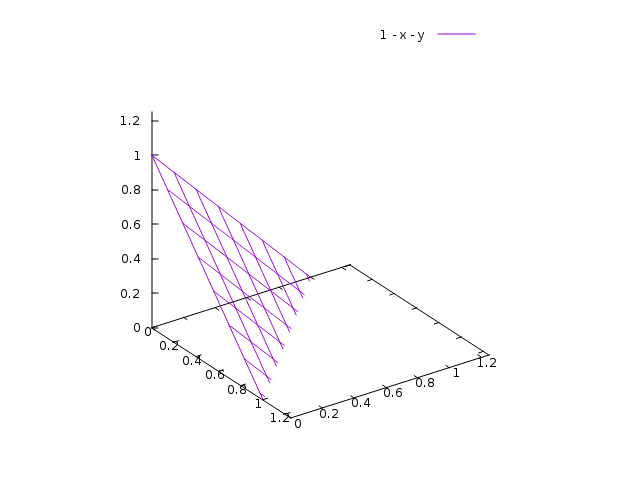
\includegraphics[scale=0.8]{xyz}	
	\end{center}

	Como esse problema não está no formato padrão, temos que reformulá-lo adicionando uma variável de folga:
	\begin{center}	
    	\begin{tabular}{r l}
	  		minimizar & $x_1 + x_2 + x_3$ \\
        
        	sujeito a & $x_1 + x_2 + x_3 + x_4 = 1$ \\
            & $x \geq 0$ \\
        \end{tabular}
    \end{center}
    
    Para esse problema, temos: 
	   
	\begin{itemize}
	\item $A = \begin{pmatrix}
    1 & 1 & 1 & 1
    \end{pmatrix}$
    
	\item $b = \begin{pmatrix}
    1 
    \end{pmatrix} $
    
    \item $c = \begin{pmatrix}
    1 & 1 & 1 & 0
    \end{pmatrix}$
    
    \item $m = 1$
    
    \item $n = 4$
	\end{itemize}
	
	Portanto, podemos aplicar nosso algoritmo:
	\begin{lstlisting}[style=term]
octave:1> simplex(A,b,c,m,n)

******************** Fase1 ********************


Iteracao 0:
|  Var Basicas       Valor
|  ===========  ==========
|           x5    1.000000
|  
|  Custo em x
|  ==========
|       1.000
|  

Iteracao 1:
|  Var Basicas       Valor
|  ===========  ==========
|           x1    1.000000
|  
|  Indice var basicas   Componente da direcao
|  ==================   =====================
|                   1               -1.000000
|  
|  Custo em x      Teta         Entra na Base   Sai da Base
|  ==========   ==========      =============   ===========
|       0.000        1.000                 x1            x5
|  
	\end{lstlisting}
	
	A fase 1 consiste em achar uma solução para o problema principal através de um problema auxiliar. Nesse caso o problema auxiliar tem somente uma variável a mais ($x_5$), pois $m = 1$. Por esse motivo, na Iteração 0, $x_5$ está na base e vale $b = 1$. Nessa situação, $c^Tx = x_5  = 1$. Como essa não é uma solução ótima, foi encontrada uma direção em que o custo reduzido é menor que 0. Vemos na Iteração 1: que essa direção é onde $j = 1$. Verificamos que $\overline{c}_j = c_j - c_B^TB^{-1}A_j = 0 - 1*1*1 = -1$. $x + \theta d$ é calculado resultando em $x_5 = 0$ e $x_1 = 1$. Nesse novo ponto, o custo vale 0. Nesse ponto, todos os custos reduzidos são maiores ou iguais a 0, e essa é a solução ótima. Como $x_1$ não é uma variável artificial, essa já é a solução inicial para o problema inicial. 
	
	\lstset {firstnumber=29}
	\begin{lstlisting}[style=term]

******************** Fase2 ********************


Iteracao 0:
|  Var Basicas       Valor
|  ===========  ==========
|           x1    1.000000
|  
|  Custo em x
|  ==========
|       1.000
|  

Iteracao 1:
|  Var Basicas       Valor
|  ===========  ==========
|           x4    1.000000
|  
|  Indice var basicas   Componente da direcao
|  ==================   =====================
|                   4               -1.000000
|  
|  Custo em x      Teta         Entra na Base   Sai da Base
|  ==========   ==========      =============   ===========
|       0.000        1.000                 x4            x1
|  


Solucao encontrada: 
x = 

   0
   0
   0
   1
	\end{lstlisting}
	
	A Iteração 0 da fase 2 começa com $x_1 = 1$, pois foi a solução inicial encontrada na Fase 1. A figura a seguir ilustra a situação:
	
	\begin{center}
	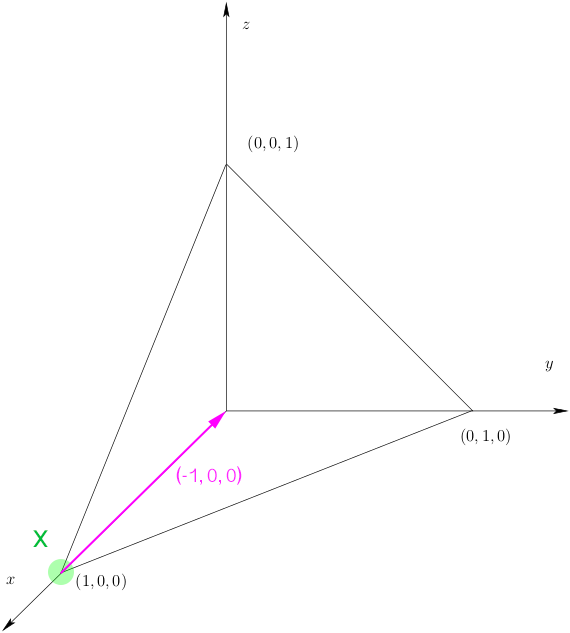
\includegraphics[scale=0.6]{xyz2}	
	\end{center}
	
	Na Iteração 1, a direção $j = 4$ é escolhida por ter custo reduzido menor que 0. Assim, $x_4$ entra na base e $x_1$ a deixa. No novo ponto onde $x_4 = 1$ e as demais componentes de x são 0, não há custo reduzido menor que 0, portanto essa é a solução ótima para nosso problema.
	
	\subsection{Custo ótimo $-\infty$}
	Suponha o problema:
	\begin{center}	
    	\begin{tabular}{r l}
	  		minimizar & $-x_1 - x_3$ \\
        
        	sujeito a & $x_1 + x_2 = 1$ \\
            & $x \geq 0$ \\
        \end{tabular}
    \end{center}
    
        Para esse problema, temos: 
	   
	\begin{itemize}
	\item $A = \begin{pmatrix}
    1 & 1 & 0 & 0
    \end{pmatrix}$
    
	\item $b = \begin{pmatrix}
    1 
    \end{pmatrix} $
    
    \item $c = \begin{pmatrix}
    -1 & 0 & -1 & 0
    \end{pmatrix}$
    
    \item $m = 1$
    
    \item $n = 3$
	\end{itemize}

	\lstset {firstnumber=1}	
	
	É fácil ver que como a unica restrição em $x_3$ é $x_3 > 0$, e temos que minimizar $-x_1 - x_3$, $x_3$ pode ser tão grande quanto queiramos e portanto o custo ótimo será $-\infty$.
	\begin{lstlisting}[style=term]
octave:1> simplex(A,b,c,m,n)

******************** Fase1 ********************


Iteracao 0:
|  Var Basicas       Valor
|  ===========  ==========
|           x4    1.000000
|  
|  Custo em x
|  ==========
|       1.000
|  

Iteracao 1:
|  Var Basicas       Valor
|  ===========  ==========
|           x1    1.000000
|  
|  Indice var basicas   Componente da direcao
|  ==================   =====================
|                   1               -1.000000
|  
|  Custo em x      Teta         Entra na Base   Sai da Base
|  ==========   ==========      =============   ===========
|       0.000        1.000                 x1            x4
|  

	\end{lstlisting}
	Como $m = 1$, a unica variável artificial será $x_4$, por isso na Iteração 0 da Fase 1, ela é a unica variável na base. No entanto na direção $j = 1$, o custo reduzido é menor que 0, portanto a variável $x_4$ sai da base e a $x_1$ entra. Nesse novo ponto, os custos reduzidos são maiores ou iguais a zero e não há variáveis artificiais na base. Assim, $x = (1, 0, 0, 0)^T$ é solução inicial do problema.
	
	\lstset {firstnumber=29}
	\begin{lstlisting}[style=term]

******************** Fase2 ********************


Iteracao 0:
|  Var Basicas       Valor
|  ===========  ==========
|           x1    1.000000
|  
|  Custo em x
|  ==========
|      -1.000
|  


O custo otimo e -infinito, com direcao:
d =

  -0
   0
   1
A partir de:
x = 

   1
   0
   0

	\end{lstlisting}
	O problema começa 

    

\newpage
\begin{thebibliography}{9}
\bibitem{315book} Dimitris Bertsimas, John N. Tsitsiklis. Introduction to Linear Optimization. 1997.
\end{thebibliography}
\end{document}

